\chapter[Dataset and Simulation][Dataset and Simulation]{Dataset and Simulation}

\section{Data}

\subsection{The 2012 Dataset} 

The LHC successfully produced datasets for physics studies in 2010, 2011 and 2012. The 2012 
proton-proton dataset was delivered with collisions with a CME of 8 TeV with bunch collisions
every 50 ns and reached a total integrated luminosity of around ~20 fb$^-1$ \cite{Aad:2013ucp}.
Figure\ref{figure:data_lumi} shows the accumulation of this dataset over time. 
Despite doubling the bunch spacing (thereby halving the bunch collision frequency), the lumonisty neared
the design lumonisty due to unexpected improvements in the transverse beam profile\cite{Carli:1424362}. This increased
the amout of pile-up, or number of collisions per bunch crossing and in general collision
events were busier due to these multiple interactions. Figure \ref{figure:data_pileup} shows
the average number of interaction per bunch crossing for the 2011 and 2012 datasets. The 2012
dataset shows an average of 20-25 interactions. 
\begin{figure}[!t]
\centering 
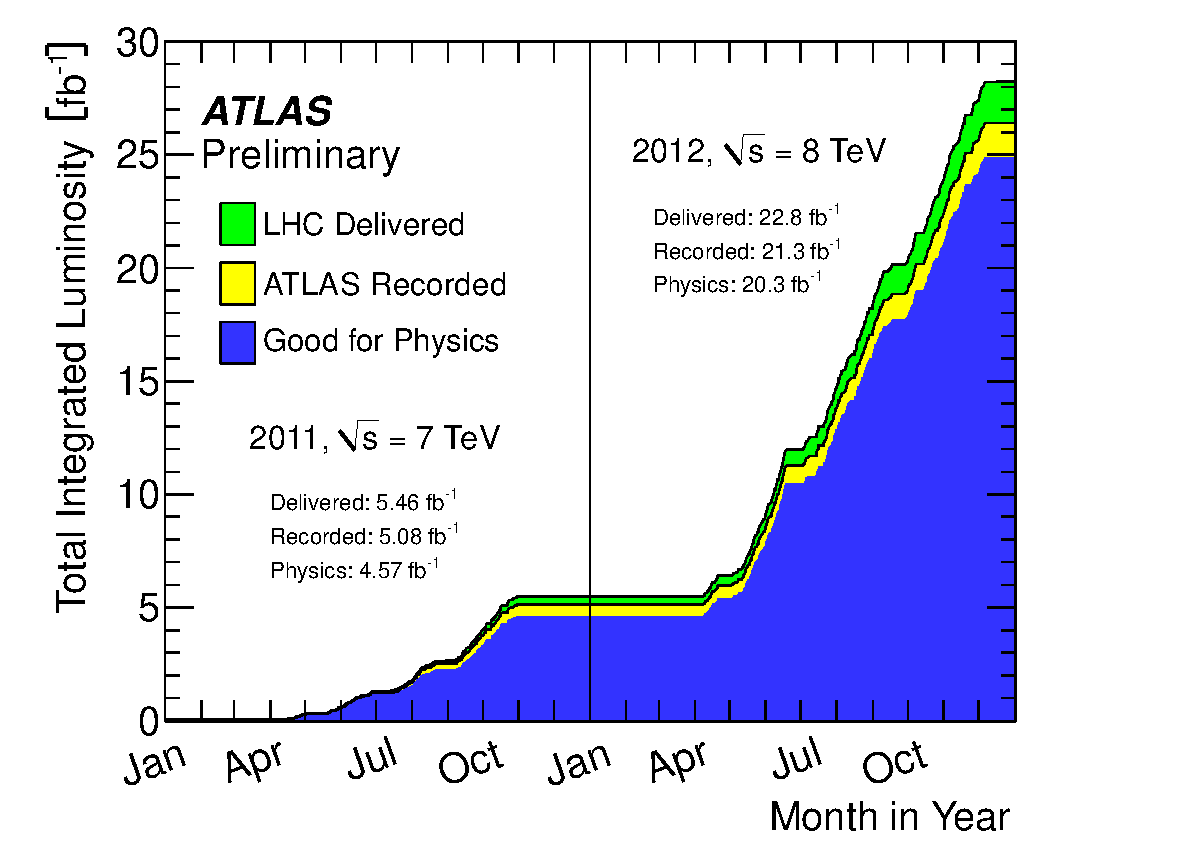
\includegraphics[width=0.60\textwidth]{figs/intlumivstime2011-2012DQ.pdf}
\caption{ Plot showing the accumulation of the integrated lumonisity delivered to the ATLAS experiment over 2011 and 2012. The rough size of the usable, physics ready dataset for 2012 is 20 $fb^-1$ and is the dataset used for the following analysis. 
}
\label{figure:data_lumi}
\end{figure}


\begin{figure}[!t]
\centering 
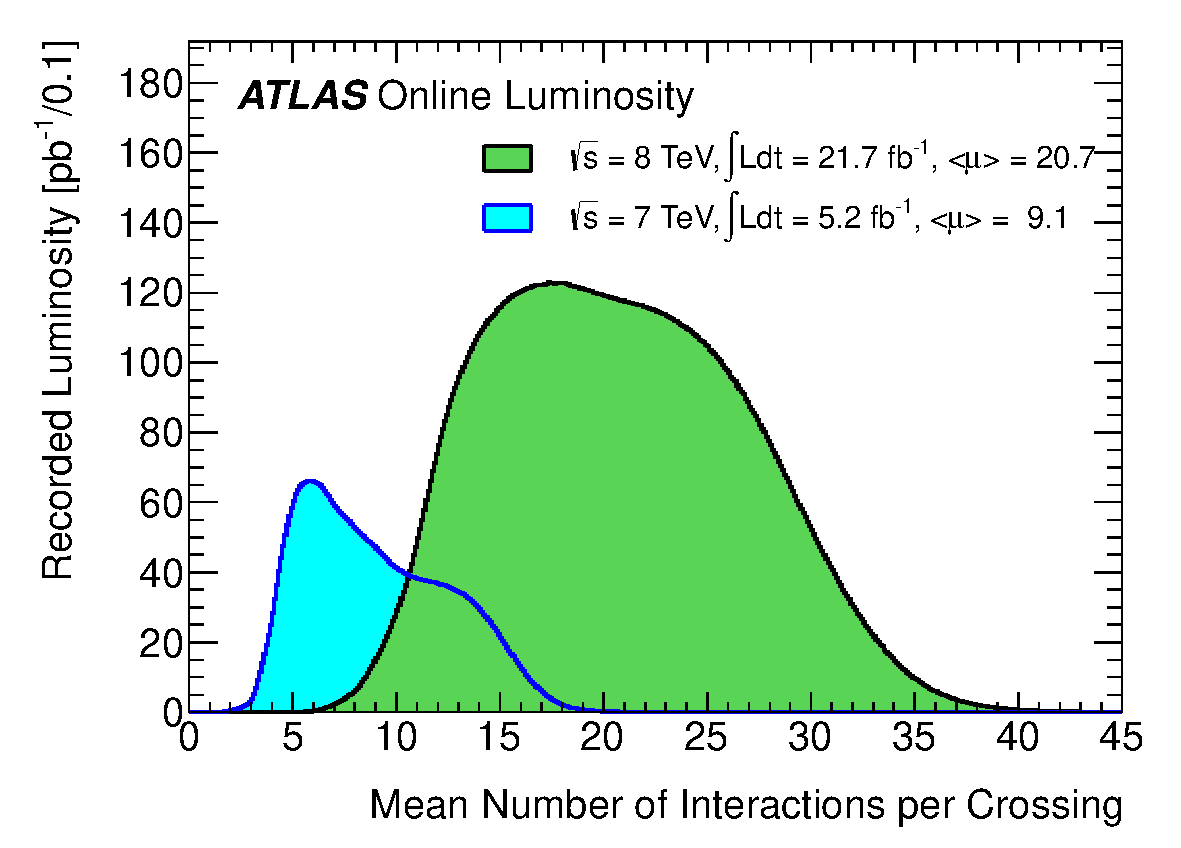
\includegraphics[width=0.60\textwidth]{figs/mu_2011_2012-dec.pdf}
\caption{ The average number of interactions per bunch-crossing for the 2012 and 2011 LHC proton-proton dataset. Most of these interactions are unintersting but leave energetic signatures in particle detectors called pile-up which interfere with measurements}\label{figure:data_pileup}
\end{figure} 

The \tth analysis uses the entire 2012 ATLAS dataset, collected
from April to December. The size of the dataset corresponds to 20.3 \ifb, after passing data quality
requirements, ensuring the proper operation of the tracking, calorimeter and muon subsystems.  

The datasets used in the analysis were collected with the primary electron
(EF\_e24vhi\_medium1 || EF\_e60\_medium1) and muon triggers (
    EF\_24i\_tight || EF\_36\_tight). The electron triggers require a electron
with at least 25 \gev\ of calorimeter energy, passing the medium identification
requirement and loose tracking isolation.  Above 60\gev, the isolation
requirement is dropped and the identification is loosened slightly. Similarly,
            the muon trigger requires a good inner detector track and matching
            hits in the muon spectrometer, as well as loose tracking isolation,
            which also is dropped about 36 \gev\.  The data sample must contain
            either a primary muon or primary electron trigger. 

\section{Simulation}

Simulation samples based on are used to determine the 
overall event selection acceptance and efficiency and for investigations not directly invovled
in the final result The simulated samples are created using parton distribution function (PDF) and
model using Monte Carlo (MC) techniques the hard parton scatter, underlying event activity and parton showering and hadronization. 
The samples are then passed through a full ATLAS detector simulation\cite{Aad:2010ah} based on  GEANT4 \cite{Agostinelli:2002hh}.
Small corrections are then applied to the overall efficiencies to re-scale object identification efficiencies,
      energy scales, and the pile-up, discussed in depth later.  

\subsection{Signal Simulation}

The signal Monte Carlo samples are described in Table~\ref{table:data_mcsignal}.
These large samples are generated with inclusive Higgs boson decays, with
branching fractions set to the LHC Higgs Cross Section Working Group (Yellow Report)
recommendation for $m_H = 125$ GeV \cite{Heinemeyer:2013tqa}.  The matrix
element calculation is performed at next-to-leading order (NLO); we use $t\bar t H$ Les Houches event format files
provided by the authors of the PowHel software \cite{Garzelli:2012zfa}, decayed and showered with
Pythia8\cite{Sjostrand:2007gs}.  The CT10\cite{Lai:2010vv} parton distribution function is used for matrix element
generation.  The inclusive cross section (129.3
fb at $m_H = 125$ GeV) is also obtained from the Yellow Report \cite{Heinemeyer:2013tqa}.
\begin{table}
\begin{center} 
    \caption{Monte Carlo samples used for signal description.}\label{table:data_mcsignal}
   \begin{tabular}{l|c|c|c|c} 

      \hline\hline
       Process & Generator & Cross- & $\mathcal{L}$ [\ifb]  & Detector \\ 
               &           & section [fb] &            &  simulation \\
\hline
 ttH$\rightarrow$allhad+H & PowHel+Pythia8 & 59.09 & 2146.5 & Full \\
 ttH$\rightarrow$ljets+H & PowHel+Pythia8 & 56.63 & 2238.9 & Full \\
 ttH$\rightarrow$ll+H & PowHel+Pythia8 & 13.58 & 9332.0 & Full \\
\hline\hline
    \end{tabular}
  \end{center}
\end{table}


\subsection{Background Simulation}

The background simulations used for this analysis are listed in
Table~\ref{table:data_MCbackground}.  In general, the Alpgen\cite{Mangano:2002ea}, MadGraph\cite{Maltoni:2002qb}, and AcerMC\cite{Kersevan:2004yg} samples use the CTEQ6L1\cite{Nadolsky:2008zw}
parton distribution function, while the Powheg\cite{Frixione:2007vw}, Sherpa\cite{Gleisberg:2008ta}, are generated with the CT10 PDF.  The exception is the MadGraph $t\bar t t \bar t$ sample, which is generated with the
MSTW2008 PDF\cite{Martin:2009iq}. The highest order calculations available are used for cross
sections.  


\begin{table}
\begin{center} 
    \caption{Monte Carlo samples used for background
      description.  Unless otherwise specified MadGraph samples use Pythia 6
      for showering and Alpgen samples use Herwig+Jimmy.}\label{table:data_MCbackground}

\begin{tabular}{l|l|c}
      \hline\hline
       Process & Generator   & Detector \\ 
               &             &  simulation \\
      \hline\hline
\ttW,\ttZ & MadGraph & Full \\
\tZ       & MadGraph & AF2 \\
$t\bar t t \bar t$ & MadGraph & Full \\
\ttWW & Madgraph+Pythia8  & AF2 \\
\ttbar & Powheg+Pythia6  & Full/AF2 \\
single top tchan & AcerMC+Pythia6& Full \\
single top schan$\rightarrow$l   & Powheg+Pythia6 & Full \\
single top $W^{\pm}t$ & Powheg+Pythia6 & Full \\
W$\gamma$*& MadGraph & Full \\
W$\gamma$+4p & Alpgen & Full \\
\WW & Sherpa &  Full \\
\WZ & Sherpa &  Full \\
Same-sign WW & Madgraph+Pythia8 & AF2 \\
ZZ$\rightarrow$ & Powheg+Pythia8,gg2ZZ+Herwig & Full \\
Z$\gamma$*  & Sherpa  & Full \\
Z+jets & Sherpa & Full \\
ggF\_H(125) & Powheg+Pythia8 & Full \\
\end{tabular}
\end{center}
\end{table}


